\documentclass[11pt,a4paper]{article}

% --- Encoding and fonts ---
\usepackage[utf8]{inputenc}
\usepackage[T1]{fontenc}
\usepackage{lmodern}

% --- Math & symbols ---
\usepackage{amsmath,amssymb,amsfonts}
\usepackage{bm}

% --- Layout & graphics ---
\usepackage[a4paper,margin=2.5cm]{geometry}
\usepackage{graphicx}
\usepackage{booktabs}
\usepackage{siunitx}

% --- Hyperlinks ---
\usepackage[colorlinks=true,linkcolor=blue,citecolor=blue,urlcolor=blue]{hyperref}

% --- Author/affiliation ---
\usepackage{authblk}
\usepackage{orcidlink}

% --- Misc ---
\numberwithin{equation}{section}

\title{\bfseries
Scale--Dependent Spacetime Geometry:\\
An Effective Field Theory Framework for Quantum--Gravity Tests Across Multiple Scales
}

\author[1]{Facundo Firmenich\,\orcidlink{0009-0002-6578-3811}}
\author[1]{Pau Firmenich}
\author[1]{Le\'on Firmenich}

\affil[1]{Centro de Estudios del Sur (CEDESUR), Buenos Aires--Barcelona}
\affil[ ]{\texttt{f.firmenich@cedesur.org}}

\date{} % leave empty for arXiv style

\begin{document}
\maketitle

\begin{abstract}
We present an effective field theory framework for testing scale--dependent 
modifications to spacetime geometry motivated by quantum gravity. For static, 
spherically symmetric configurations, we construct a set of benchmark metric 
ans\"atze (Yukawa--type, power--law, RG--improved) that capture leading deviations 
from GR induced by running couplings, discrete structure, or higher--curvature 
interactions. We derive explicit mappings to the Parameterized Post--Newtonian (PPN) 
and parameterized post--Einsteinian (ppE) formalisms and provide analytic expressions 
for perihelion precession, light deflection, and gravitational--wave phasing. 
As a worked example, we present a Gaia--like forecast for Yukawa--type modifications 
and discuss how Cassini, ephemerides, torsion--balance, and binary--pulsar bounds 
can be combined in a single parameter space. A Python toolkit implementing the main 
ans\"atze and observables is provided to facilitate reproducible phenomenology. 
This framework enables systematic searches within a representative set of 
scale--dependent parameterizations motivated by quantum gravity across solar--system, 
binary--pulsar, and gravitational--wave data.
\end{abstract}

\section{Introduction}
\label{sec:intro}

The empirical detection of quantum--gravity effects remains one of the central open 
challenges in fundamental physics. General relativity (GR) has been exquisitely 
tested in the solar system, with Parameterized Post--Newtonian (PPN) bounds on the 
Eddington parameter $\gamma$ at the level $|1-\gamma|\lesssim 10^{-5}$ and comparable 
constraints on other PPN parameters~\cite{Will2014,Will2018}. Gravitational--wave 
observations, binary pulsars, lunar laser ranging, and sub--millimeter tests of the 
inverse--square law further support GR across a wide range of scales and regimes
from weak--field, slow--motion dynamics to the genuinely relativistic inspiral of 
compact objects~\cite{BertottiIessTortora2003,Weisberg2016,Freire2012,Abbott2021,Adelberger2009,Williams2018,Murphy2013}.

Despite this success, a variety of quantum--gravity approaches predict that spacetime 
acquires a nontrivial \emph{scale dependence}. In asymptotically safe quantum gravity, 
gravitational couplings run under the renormalization group and lead to effective metrics 
that depend on the probing scale~\cite{ReuterSaueressig2012}. Loop quantum gravity suggests 
discrete spectra for areas and volumes, with a fundamental area gap that may induce effective 
modifications at small scales~\cite{Rovelli2004,AshtekarBojowald2005}. Non--commutative geometry 
introduces a fundamental length scale through non--vanishing commutators of coordinates and 
smearing of point sources~\cite{Connes1994,SeibergWitten1999,Nicolini2006,Ansoldi2008}. 
Effective field theory (EFT) treatments of GR naturally produce higher--curvature terms 
that, when resummed or evaluated at finite scales, can be encoded as corrections to 
metric components~\cite{Donoghue1994,Burgess2004,Stelle1978,Accioly2002}.

In all these settings, the notion of \emph{scale} arises in partially complementary ways:
\begin{itemize}
  \item a resolution scale associated with the probe (e.g.\ angular or temporal resolution in an experiment);
  \item an energy or momentum scale $k$ entering renormalization--group flows or scattering amplitudes;
  \item a geometric scale (e.g.\ radial distance in a spherically symmetric configuration).
\end{itemize}
This motivates the more general notion of \emph{scale--dependent spacetime geometry}, 
where the effective metric sensed by a given experiment depends on the relevant observational scale.

The objective of this paper is to provide a \emph{phenomenological framework} that captures 
such scale dependence in a way that is:
\begin{enumerate}
  \item anchored in effective field theory;
  \item systematically expandable and falsifiable;
  \item compatible with existing PPN and ppE parameterizations, while extending them in directions motivated by quantum gravity;
  \item directly usable in the analysis of current and future data.
\end{enumerate}

The spirit is similar to the parameterized post--Einsteinian (ppE) framework for gravitational 
waves~\cite{YunesPretorius2009,YunesSiemens2013} or the various cosmological parameterized 
modified gravity schemes~\cite{Clifton2012,Joyce2015}, but focused on \emph{scale--dependent, 
spherically symmetric} configurations with direct relevance to solar--system and strong--field tests.

This paper is organized as follows. In Sec.~\ref{sec:metric} we introduce our scale--dependent metric 
parameterization, fix a convenient gauge, and define a set of benchmark ans\"atze. In Sec.~\ref{sec:EFT} 
we connect these ans\"atze to the EFT of gravity, asymptotic safety, loop quantum gravity, and 
non--commutative geometry. In Sec.~\ref{sec:obs} we derive the Newtonian and post--Newtonian limits, 
map to PPN parameters, and obtain expressions for key observables. Sec.~\ref{sec:multiprobe} discusses 
multi--probe sensitivities and parameter degeneracies. Sec.~\ref{sec:gaia} presents a worked example 
of Gaia--like constraints on a Yukawa--type scale--dependent metric. Sec.~\ref{sec:energy} discusses 
consistency and energy conditions, with technical details in Appendix~\ref{app:energy}. We conclude in 
Sec.~\ref{sec:disc}. Additional derivations for orbital and light--propagation observables, including 
explicit integral formulas for Yukawa--type corrections, are collected in Appendix~\ref{app:orbits}.

\section{Scale--Dependent Spherically Symmetric Metrics}
\label{sec:metric}

\subsection{General setup and gauge choice}

We consider static, spherically symmetric spptimes of the general form
\begin{equation}
  ds^2 = -c^2 A(r)\,dt^2 + B(r)\,dr^2 + r^2 C(r)\,d\Omega^2,
  \label{eq:metric-ABC}
\end{equation}
where $d\Omega^2 = d\theta^2 + \sin^2\theta\,d\varphi^2$, and $A(r)$, $B(r)$, $C(r)$ are positive 
functions encoding deviations from the Schwarzschild solution. 

As is well known, there is residual gauge freedom in the radial coordinate. For static, spherically 
symmetric metrics, one can always redefine $r$ such that $C(r)\equiv 1$, in which case $r$ coincides 
with the areal radius. We adopt this gauge:
\begin{equation}
  ds^2 = -c^2 A(r)\,dt^2 + B(r)\,dr^2 + r^2 d\Omega^2.
  \label{eq:metric-AB}
\end{equation}
In GR, the vacuum solution for a point mass $M$ is
\begin{equation}
  A_{\rm GR}(r) = 1 - \frac{2GM}{c^2 r}, 
  \qquad
  B_{\rm GR}(r) = \left(1 - \frac{2GM}{c^2 r}\right)^{-1}.
  \label{eq:schwarz}
\end{equation}

We model deviations from GR as
\begin{equation}
  A(r) = A_{\rm GR}(r)\left[1 + \delta A(r)\right],
  \qquad
  B(r) = B_{\rm GR}(r)\left[1 + \delta B(r)\right],
  \label{eq:deltaAB}
\end{equation}
with $\delta A,\delta B$ dimensionless functions that encode scale--dependent modifications. In 
the weak--field regime, $GM/(c^2 r)\ll 1$ and $|\delta A|,|\delta B|\ll 1$, we write
\begin{equation}
  A(r) = 1 + \frac{2\Phi(r)}{c^2} + \mathcal{O}\!\left(\frac{\Phi^2}{c^4}\right),
  \qquad
  B(r) = 1 - \frac{2\Psi(r)}{c^2} + \mathcal{O}\!\left(\frac{\Psi^2}{c^4}\right),
  \label{eq:PhiPsi}
\end{equation}
where $\Phi$ and $\Psi$ are effective gravitational potentials. In GR, $\Phi=\Psi=-GM/r$ for 
non--relativistic sources. Scale dependence will be encoded in deviations of $\Phi,\Psi$ from 
this form.

\subsection{Notation and symbols}

For convenience, Table~\ref{tab:symbols} summarizes the main symbols used throughout the paper.

\begin{table}[t]
  \centering
  \sisetup{table-format=1.1}
  \begin{tabular}{p{3.2cm}p{10cm}}
    \toprule
    Symbol & Meaning \\
    \midrule
    $\Phi(r)$, $\Psi(r)$ & Effective gravitational potentials in the weak--field metric \\
    $\delta_{\Phi}(r)$, $\delta_{\Psi}(r)$ & Fractional deviations from the Newtonian potential, Eq.~\eqref{eq:deltaPhiPsi} \\
    $\gamma_{\rm eff}(r)$ & Scale--dependent generalization of the PPN parameter $\gamma$ \\
    $\ell_{\rm s}$ & Characteristic scale of scale--dependent corrections (generic) \\
    $\alpha_{\rm Y}$, $\lambda_{\rm Y}$ & Amplitude and range of Yukawa--type corrections \\
    $\epsilon$, $\beta$ & Amplitude and power for power--law corrections \\
    $\xi$, $n$, $r_0$ & Parameters in RG--improved running $G(r)$ \\
    $a$, $e$ & Semi--major axis and eccentricity of a bound orbit \\
    $b$ & Impact parameter for light deflection \\
    $M$ & Central mass (e.g.\ solar mass $M_\odot$) \\
    $R_{\rm S}$ & Schwarzschild radius $2GM/c^2$ of the central mass \\
    \bottomrule
  \end{tabular}
  \caption{Main symbols and parameters used in the text.}
  \label{tab:symbols}
\end{table}

\subsection{Benchmark ans\"atze for scale dependence}
\label{subsec:ansatze}

Quantum--gravity effects can generate corrections to the Newtonian potential and post--Newtonian 
metric that are nonlocal and scale dependent. We do not attempt to capture the full model space; 
instead, we introduce a small set of benchmark ans\"atze, each characterized by a \emph{scale 
parameter} $\ell_{\rm s}$ and one or more dimensionless amplitudes.

\subsubsection{Yukawa--type modification}

A widely used phenomenological form is a Yukawa--type correction to the Newtonian potential,
\begin{equation}
  \Phi(r) = -\frac{GM}{r}\left[1 + \alpha_{\rm Y} e^{-r/\lambda_{\rm Y}}\right],
  \label{eq:YukawaPhi}
\end{equation}
where $\alpha_{\rm Y}$ controls the strength and $\lambda_{\rm Y}$ the range of the new interaction. 
The corresponding metric functions in the weak--field regime are
\begin{equation}
  A(r) \simeq 1 + \frac{2\Phi(r)}{c^2},
  \qquad
  B(r) \simeq 1 - \frac{2\gamma_{\rm eff}(r)\,\Phi(r)}{c^2},
  \label{eq:YukawaAB}
\end{equation}
where $\gamma_{\rm eff}(r)$ generalizes the PPN parameter $\gamma$ to a (possibly) scale--dependent 
function. In minimally coupled scalar--tensor realizations, one typically has $\gamma_{\rm eff}(r)
\rightarrow 1$ at large $r$ and deviations at $r\lesssim \lambda_{\rm Y}$.

For the purposes of this framework, we treat $\alpha_{\rm Y}$ and $\lambda_{\rm Y}$ as phenomenological 
parameters. The scale $\ell_{\rm s}$ is identified with $\lambda_{\rm Y}$.

\subsubsection{Power--law modification}

Some quantum--gravity scenarios predict long--range corrections that follow a power law in radius. 
We model this via
\begin{equation}
  \Phi(r) = -\frac{GM}{r}\left[1 + \epsilon\left(\frac{r}{\ell_{\rm s}}\right)^{\beta}\right],
  \label{eq:PowerPhi}
\end{equation}
with $\epsilon$ dimensionless, $\beta$ real, and $\ell_{\rm s}$ a characteristic length scale. For 
$\beta>0$, the correction grows with $r$; for $\beta<0$, it dominates at small radii.

Again, we take
\begin{equation}
  A(r) \simeq 1 + \frac{2\Phi(r)}{c^2},
  \qquad
  B(r) \simeq 1 - \frac{2\gamma_{\rm eff}(r)\,\Phi(r)}{c^2},
  \label{eq:PowerAB}
\end{equation}
with $\gamma_{\rm eff}(r)$ parameterizing possible anisotropic stress.

\subsubsection{RG--improved (asymptotic--safety inspired) metric}

In asymptotically safe gravity, the Newton constant becomes scale dependent, $G\to G(k)$, where $k$ 
is a renormalization--group scale. A commonly used identification is $k\sim 1/d(r)$, where $d(r)$ 
is a physical distance scale (often $d\sim r$ for spherically symmetric solutions)~\cite{ReuterSaueressig2012}. 
As a simple phenomenological model, we take
\begin{equation}
  G(r) = \frac{G_0}{1 + \xi \left(\dfrac{r_0}{r}\right)^n},
  \label{eq:Gr}
\end{equation}
with $\xi$ dimensionless, $n>0$, and $r_0$ a reference scale. The effective gravitational potential 
then becomes
\begin{equation}
  \Phi(r) = -\frac{G(r) M}{r} = -\frac{G_0 M}{r}\left[1 + \xi\left(\frac{r_0}{r}\right)^n\right]^{-1}.
  \label{eq:RGPhi}
\end{equation}
For $r\gg r_0$, one recovers the standard potential up to corrections $\mathcal{O}(\xi (r_0/r)^n)$, 
while for $r\ll r_0$ the coupling saturates at $G(r)\simeq G_0/(1+\xi)$.

Equation~\eqref{eq:RGPhi} can be expanded in powers of $\xi (r_0/r)^n$ to connect with the power--law 
form~\eqref{eq:PowerPhi}. Again,
\begin{equation}
  A(r) \simeq 1 + \frac{2\Phi(r)}{c^2},
  \qquad
  B(r) \simeq 1 - \frac{2\gamma_{\rm eff}(r)\,\Phi(r)}{c^2},
\end{equation}
with $\ell_{\rm s}\sim r_0$.

\subsection{Minimal and extended $\gamma_{\rm eff}(r)$ ans\"atze}
\label{subsec:gammaeff}

The ratio
\begin{equation}
  \gamma_{\rm eff}(r) \equiv \frac{\Psi(r)}{\Phi(r)}
\end{equation}
generalizes the standard PPN parameter $\gamma$ to a scale--dependent function. In many modified 
gravity theories (e.g.\ scalar--tensor models) $\gamma_{\rm eff}(r)$ acquires a nontrivial radial 
dependence even if the underlying model has only a small number of new parameters. For our benchmark 
parameterizations, we adopt two complementary modeling strategies:
\begin{itemize}
  \item \emph{Minimal ansatz:} we set
  \begin{equation}
    \Psi(r) = \gamma_{\infty}\,\Phi(r),
  \end{equation}
  with $\gamma_{\infty}$ a constant close to unity.\footnote{Here $\gamma_{\infty}$ is not assumed 
  to be a fundamental constant of the theory, but an effective large--scale limit of 
  $\gamma_{\rm eff}(r)$ over the radial range probed by the experiment.}
  \item \emph{Extended ansatz:} we allow for
  \begin{equation}
    \gamma_{\rm eff}(r) = 1 + \delta\gamma(r),
  \end{equation}
  with $\delta\gamma(r)$ determined by the specific model (e.g.\ underlying scalar--tensor theory 
  or higher--derivative EFT) and possibly scale dependent.
\end{itemize}

It is important to emphasize that the minimal ansatz is an \emph{approximation}. In practice, it 
is self--consistent for a given observable (e.g.\ Cassini Shapiro delay) if the variation of 
$\gamma_{\rm eff}(r)$ across the region sampled by the signal is smaller than the experimental 
uncertainty. For instance, for Cassini--like measurements with sensitivity
\begin{equation}
  \left|\gamma_{\rm eff}(r_{\rm Cassini}) - 1\right| \lesssim 2.3\times 10^{-5},
\end{equation}
the minimal ansatz is acceptable if
\begin{equation}
  \left|\gamma_{\rm eff}(r_{\rm max}) - \gamma_{\rm eff}(r_{\rm min})\right|
  \ll 2.3\times 10^{-5}
\end{equation}
over the range of radii $[r_{\rm min},r_{\rm max}]$ effectively probed by the radio link. 
For specific models, this criterion can be translated into bounds on $(\alpha_{\rm Y},\lambda_{\rm Y})$ 
or $(\epsilon,\beta,\ell_{\rm s})$, by evaluating $\gamma_{\rm eff}(r)$ numerically at the relevant 
radii (e.g.\ perihelion and aphelion) and checking whether the spread is below the observational 
error bar. When this condition fails, the extended ansatz with explicit $r$--dependence in 
$\gamma_{\rm eff}(r)$ should be used.

\section{Connection to Effective Field Theory and Quantum Gravity}
\label{sec:EFT}

\subsection{Effective field theory of gravity}

In the EFT treatment of gravity, valid well below the Planck scale, the low--energy Lagrangian 
takes the form~\cite{Donoghue1994,Burgess2004,Stelle1978,Accioly2002}
\begin{equation}
  \mathcal{L}_{\rm eff} = \frac{2}{\kappa^2}\sqrt{-g}\,R 
  + \sqrt{-g}\left(
      c_1 R^2 
    + c_2 R_{\mu\nu}R^{\mu\nu}
    + c_3 R_{\mu\nu\rho\sigma}R^{\mu\nu\rho\sigma}
    + \cdots
  \right) 
  + \mathcal{L}_{\rm matter},
  \label{eq:Leff}
\end{equation}
where $\kappa^2 = 32\pi G_0/c^4$, the $c_i$ are Wilson coefficients suppressed by appropriate powers 
of the ultraviolet scale, and the ellipsis denotes higher--dimension operators and nonlocal terms 
arising from loops.

Linearizing around Minkowski and solving the field equations for a static point mass yields, 
schematically,
\begin{equation}
  \Phi(r) = -\frac{G_0 M}{r}\left[1 + \alpha_0 e^{-m_0 r} + \alpha_2 e^{-m_2 r} + \cdots\right],
  \label{eq:EFTPhi}
\end{equation}
where $m_0^{-1}$ and $m_2^{-1}$ are length scales associated with massive scalar and tensor modes 
introduced by the higher--curvature terms, and $\alpha_0,\alpha_2$ are dimensionless coefficients 
determined by the $c_i$ (see, e.g.,~\cite{Stelle1978,Accioly2002}). This is precisely of Yukawa 
form \eqref{eq:YukawaPhi}, with
\begin{equation}
  \alpha_{\rm Y} \leftrightarrow \alpha_0,\alpha_2,
  \qquad
  \lambda_{\rm Y} \leftrightarrow m_0^{-1},m_2^{-1}.
\end{equation}
Thus, the Yukawa ansatz~\eqref{eq:YukawaPhi} is directly motivated by the EFT of gravity. The EFT 
also predicts logarithmic and nonlocal corrections at long distances, which can be modeled by 
power--law or more general functional forms.

\subsection{Asymptotic safety and RG--improved metrics}

In the asymptotic safety program, the gravitational couplings run to a nontrivial ultraviolet fixed 
point under the renormalization group. In truncated flows, one often finds
\begin{equation}
  G(k) = \frac{G_0}{1 + \omega G_0 k^2},
  \label{eq:Gk}
\end{equation}
with $\omega>0$ a parameter in the truncation~\cite{ReuterSaueressig2012}. A standard phenomenological 
strategy is to identify the RG scale $k$ with an inverse length scale, $k\sim 1/d(r)$, where $d(r)$ is 
a physical distance in the background geometry. Several prescriptions have been proposed, for example
\begin{equation}
  k(r) \sim \frac{1}{r}, \qquad
  k^4(r) \sim K(r) \equiv R_{\mu\nu\rho\sigma}R^{\mu\nu\rho\sigma},
\end{equation}
where $K$ is the Kretschmann scalar evaluated on a zeroth--order (e.g.\ Schwarzschild) solution. 
Each choice defines a different ``RG--improvement scheme'' and leads to a different $G(r)$. When 
mapping observational bounds onto $(\xi,n,r_0)$ in Eq.~\eqref{eq:Gr}, one should bear in mind that 
the resulting constraints are, strictly speaking, constraints on the combination of $G(k)$ and the 
chosen $k(r)$ prescription. 

In practice, phenomenological analyses can proceed by adopting one or two representative prescriptions 
(e.g.\ $k\sim 1/r$ and $k^4\sim K$), computing the corresponding $G(r)$, and treating the spread in 
resulting bounds as a measure of theoretical scheme dependence. Our framework is designed so that 
this scheme dependence can be tracked explicitly within the same parameterization.

\subsection{Loop quantum gravity and non--commutative geometry}

In loop quantum gravity, the area operator has a minimum nonzero eigenvalue (the area gap), which 
introduces a fundamental scale $\ell_{\rm LQG}\sim \sqrt{\Delta}$~\cite{Rovelli2004,AshtekarBojowald2005}. 
Effective models that coarse--grain the discrete structure can produce corrections to the metric 
components that become relevant when $r\sim \ell_{\rm LQG}$; these can be encoded in either 
Yukawa--like or power--law terms in $\Phi(r)$ and $\Psi(r)$.

Non--commutative geometry introduces a scale $\sqrt{\theta}$ through commutators $[x^\mu,x^\nu]
\sim i\theta^{\mu\nu}$~\cite{Connes1994,SeibergWitten1999}. In simple spherically symmetric models, 
this leads to an effective smearing of point sources and regular black holes with Gaussian--type 
mass distributions~\cite{Nicolini2006,Ansoldi2008}. Again, this can be represented via suitable 
choices of $\Phi(r)$ and $\Psi(r)$ within our ansatz.

We stress that our goal is not to derive these corrections from first principles, but to provide a 
\emph{common language} in which their observable consequences can be parameterized and constrained.

\section{Observables and Mapping to Existing Frameworks}
\label{sec:obs}

\subsection{Newtonian limit and potentials}

In the weak--field, slow--motion limit, test particles follow trajectories determined by the effective 
Newtonian potential $\Phi(r)$:
\begin{equation}
  \frac{d^2\bm{x}}{dt^2} = -\nabla\Phi(\bm{x}) + \mathcal{O}\!\left(\frac{v^2}{c^2}\right).
\end{equation}
Given a choice of ansatz for $\Phi(r)$, the corrections to Keplerian orbits, epicyclic frequencies, 
and other Newtonian observables follow straightforwardly.

For later use, we define
\begin{equation}
  \Phi(r) = -\frac{G_0 M}{r}\left[1 + \delta_{\Phi}(r)\right],
  \qquad
  \Psi(r) = -\frac{G_0 M}{r}\left[1 + \delta_{\Psi}(r)\right],
  \label{eq:deltaPhiPsi}
\end{equation}
where $\delta_{\Phi}$ and $\delta_{\Psi}$ encode deviations from GR. In GR, $\delta_{\Phi}=\delta_{\Psi}=0$ 
for a point mass in vacuum.

\subsection{Post--Newtonian expansion and PPN mapping}

The Parameterized Post--Newtonian formalism expresses the metric around a slowly moving gravitating 
source in terms of a set of parameters $(\gamma,\beta,\xi,\dots)$ that capture possible deviations 
from GR at first post--Newtonian order~\cite{Will2014,Will2018}. For a static, spherically symmetric 
configuration, the line element in isotropic coordinates is
\begin{align}
  g_{tt} &= -c^2\left[1 - 2\frac{U}{c^2} + 2\beta\frac{U^2}{c^4} + \mathcal{O}\!\left(\frac{U^3}{c^6}\right)\right],
  \label{eq:PPN-tt} \\
  g_{rr} &= 1 + 2\gamma\frac{U}{c^2} + \mathcal{O}\!\left(\frac{U^2}{c^4}\right),
  \label{eq:PPN-rr}
\end{align}
where $U(\bm{x})$ is the Newtonian potential. Comparing with our parameterization \eqref{eq:PhiPsi}, 
we identify, in the weak--field regime,
\begin{equation}
  \Phi(r) = U(r) + \mathcal{O}\!\left(\frac{U^2}{c^2}\right),
  \qquad
  \Psi(r) = \gamma_{\rm eff}(r) U(r),
\end{equation}
with
\begin{equation}
  \gamma_{\rm eff}(r) \equiv \frac{\Psi(r)}{\Phi(r)}
  = \frac{1 + \delta_{\Psi}(r)}{1 + \delta_{\Phi}(r)}.
\end{equation}
If $\gamma_{\rm eff}(r)$ tends to a constant $\gamma$ as $r\to\infty$ and the metric is analytic in 
$U$, then our framework reproduces standard PPN at large radii, with
\begin{equation}
  \gamma = \lim_{r\to\infty}\gamma_{\rm eff}(r),
  \qquad
  \beta = \text{coefficient of } U^2 \text{ in } g_{tt}.
\end{equation}
In the ans\"atze considered in Sec.~\ref{subsec:ansatze}, we have explicitly imposed a linear weak--field 
form,
\begin{equation}
  A(r) \simeq 1 + \frac{2\Phi(r)}{c^2},
  \qquad
  B(r) \simeq 1 - \frac{2\Psi(r)}{c^2},
\end{equation}
without including explicit $U^2$ terms. In this restricted setting, the leading post--Newtonian 
parameter is $\gamma_{\rm eff}(r)$, while $\beta_{\rm eff}(r)$ remains equal to unity at the order 
we consider. A more general parameterization could promote $\beta_{\rm eff}(r)$ to a scale--dependent 
function by including explicit $U^2$ contributions in $A(r)$.

We therefore parameterize
\begin{equation}
  \gamma_{\rm eff}(r) = \gamma + \delta \gamma(r),
  \qquad
  \beta_{\rm eff}(r) = 1 + \delta \beta(r),
\end{equation}
where $\delta\gamma,\delta\beta$ vanish at scales where classical PPN tests have already constrained 
deviations. For a given ansatz (e.g.\ Yukawa or power law), one can expand the metric in powers of 
$U$ and read off $\gamma_{\rm eff}(r)$ and $\beta_{\rm eff}(r)$ explicitly.

\subsection{Solar--system and binary--pulsar observables}
\label{subsec:ss-binary}

We briefly summarize the leading corrections to key observables in terms of $\Phi(r)$ and $\Psi(r)$. 
Detailed derivations for test particles in the metric~\eqref{eq:metric-AB} are provided in 
Appendix~\ref{app:orbits}.

\subsubsection{Perihelion precession}

For a nearly Keplerian orbit with semi--major axis $a$ and eccentricity $e$ in a central potential 
$\Phi(r)$, the anomalous perihelion precession per orbit can be expressed as~\cite{AdkinsMcDonnell2007}
\begin{equation}
  \Delta\varpi \simeq -\frac{1}{na^2 e}\frac{\partial}{\partial e}\left\langle \delta \Phi(r)\right\rangle,
  \label{eq:perihelion-general}
\end{equation}
where $n=\sqrt{G_0 M/a^3}$ is the mean motion, $\delta\Phi(r)\equiv \Phi(r)+G_0 M/r$ is the deviation 
from the Newtonian potential, and $\langle \cdot\rangle$ denotes an average over one orbit. For the GR 
correction from the Schwarzschild metric, this reproduces the standard
\begin{equation}
  \Delta\varpi_{\rm GR} = \frac{6\pi G_0 M}{c^2 a(1-e^2)}.
\end{equation}
For a Yukawa correction~\eqref{eq:YukawaPhi}, inserting $\delta\Phi(r)$ into Eq.~\eqref{eq:perihelion-general} 
yields an additional contribution $\Delta\varpi_{\rm Y}(\alpha_{\rm Y},\lambda_{\rm Y})$ that can be 
expressed in terms of a one--dimensional integral over the orbital true anomaly; see Appendix~\ref{app:orbits} 
for explicit formulas. Ephemerides analyses, e.g.\ INPOP13c, constrain such deviations at the level 
$|\Delta\varpi_{\rm Y}/\Delta\varpi_{\rm GR}|\lesssim 10^{-4}$ for Mercury--like orbits~\cite{Verma2014}.

\subsubsection{Light deflection and Shapiro time delay}

To leading order, the deflection angle of a light ray with impact parameter $b$ in the 
metric~\eqref{eq:metric-AB} is
\begin{equation}
  \hat{\alpha}(b) \simeq \frac{2}{c^2}\int_{-\infty}^{+\infty} 
  \left[\nabla_{\perp} \left(\Phi + \Psi\right)\right] dz
  = \frac{4G_0 M_{\rm lens}(b)}{c^2 b}\left[1 + \delta_{\rm defl}(b)\right],
  \label{eq:deflection-general}
\end{equation}
where $z$ is the coordinate along the line of sight, $\nabla_{\perp}$ is the gradient in the transverse 
plane, and $M_{\rm lens}(b)$ is the mass enclosed within the impact parameter $b$. In GR with 
$\Phi=\Psi=-G_0 M/r$, one has $\delta_{\rm defl}=0$. Scale--dependent corrections enter through 
$\delta_{\Phi},\delta_{\Psi}$ in Eq.~\eqref{eq:deltaPhiPsi} and a possible scale dependence of 
$\gamma_{\rm eff}(r)$.

The Shapiro time delay for a signal propagating past a mass $M$ acquires a correction proportional to 
$(1+\gamma_{\rm eff})$; Cassini--like experiments constrain combinations of $\delta_{\Phi},\delta_{\Psi}$ 
at solar--system scales~\cite{BertottiIessTortora2003}. While the original Cassini result was obtained 
via Shapiro delay, the constraint on $\gamma$ also applies to light deflection at similar scales. In our 
framework, this can be recast as a bound on $\gamma_{\rm eff}(r)$ evaluated at Cassini--like impact 
parameters ($\sim 1.6 R_\odot$) and heliocentric distances ($\sim 1$--$8$\,AU),
\begin{equation}
  \left|\gamma_{\rm eff}(r_{\rm Cassini}) - 1\right| \lesssim 2.3\times 10^{-5}.
\end{equation}

\subsubsection{Orbital decay in binary systems}

Energy loss via gravitational radiation leads to orbital decay in binary pulsars. In GR, the orbital 
period derivative $\dot{P}_b$ is determined by the quadrupole formula. Modifications of the metric and 
of the gravitational radiation sector can be parameterized by a correction factor,
\begin{equation}
  \dot{P}_b = \dot{P}_b^{\rm GR} \left[1 + \delta_{\dot{P}}(\Phi,\Psi; \text{radiation sector})\right].
\end{equation}
In many models, the leading scale--dependent corrections enter through modifications to the conservative 
dynamics (encoded in $\Phi,\Psi$) and through additional radiation channels. Our framework focuses on 
the conservative part; the radiation sector can be further parameterized using ppE--like phasing 
parameters~\cite{YunesPretorius2009,YunesSiemens2013}. Binary pulsar systems such as 
PSR~B1913+16~\cite{Weisberg2016} and PSR~J1738+0333~\cite{Freire2012} bound fractional deviations 
$|\delta\dot{P}_b/\dot{P}_b^{\rm GR}|\lesssim 10^{-6}$--$10^{-7}$, but the detailed interpretation 
of these bounds in a scale--dependent metric framework is strongly model--dependent and may involve 
screening mechanisms.

\subsection{Gravitational waves and ppE mapping}

In the frequency domain, the Fourier transform of the GR inspiral waveform for a compact binary can be 
written as
\begin{equation}
  \tilde{h}_{\rm GR}(f) = \mathcal{A}(f) \exp\left[i\Psi_{\rm GR}(f)\right],
\end{equation}
where $\mathcal{A}$ is the amplitude and $\Psi_{\rm GR}$ the phase. The ppE framework models 
deviations as~\cite{YunesPretorius2009,YunesSiemens2013}
\begin{equation}
  \tilde{h}(f) = \tilde{h}_{\rm GR}(f)\left[1 + \alpha_{\rm ppE} u^a\right]\exp\left[i\beta_{\rm ppE} u^b\right],
  \qquad u \equiv (\pi \mathcal{M} f)^{1/3},
  \label{eq:ppE}
\end{equation}
where $\mathcal{M}$ is the chirp mass and $(\alpha_{\rm ppE},\beta_{\rm ppE},a,b)$ encode deviations.

Scale--dependent modifications to the metric can affect both the binding energy $E$ and the 
gravitational--wave luminosity $\mathcal{F}$ of the binary. Writing
\begin{equation}
  E = E_{\rm GR}\left[1 + \delta_E(u)\right],
  \qquad
  \mathcal{F} = \mathcal{F}_{\rm GR}\left[1 + \delta_{\mathcal{F}}(u)\right],
\end{equation}
and using the balance law $dE/dt = -\mathcal{F}$, one finds that the orbital phase and, hence, the 
Fourier phase $\Psi(f)$ acquire corrections that can be expressed as a PN series,
\begin{equation}
  \Psi(f) = \Psi_{\rm GR}(f) + \sum_k \Delta\varphi_k\,u^k,
\end{equation}
where the coefficients $\Delta\varphi_k$ are determined by $\delta_E(u)$ and $\delta_{\mathcal{F}}(u)$. 
Matching this expansion to the ppE form~\eqref{eq:ppE} yields effective ppE parameters
\begin{equation}
  b = k_{\star}, \qquad 
  \beta_{\rm ppE} \propto \Delta\varphi_{k_{\star}},
\end{equation}
for those PN orders $k_{\star}$ at which the scale--dependent modification first appears. For a given 
ansatz for $\Phi,\Psi$, our framework provides a systematic way to compute $\delta_E(u)$ and 
$\delta_{\mathcal{F}}(u)$ and thus derive the corresponding ppE parameters. Current LIGO--Virgo--KAGRA 
data constrain such phasing deviations at the $\lesssim 10^{-1}$--$10^{-2}$ level over a range of PN 
orders~\cite{Abbott2021}.

\subsection{Relation to existing parameterized frameworks}

Our proposal is complementary to PPN, ppE, and cosmological parameterized modified gravity frameworks:
\begin{itemize}
  \item At the level of the metric, we reproduce PPN in the limit of scale--independent parameters 
  and provide a controlled way to introduce \emph{radial} or \emph{scale--dependent} generalizations 
  of $\gamma$ and $\beta$.
  \item At the level of gravitational--wave phasing, we provide a mapping to ppE parameters, allowing 
  the same underlying scale--dependent model to be constrained via both solar--system and binary--merger data.
  \item Our focus on static, spherically symmetric configurations complements cosmological frameworks 
  (e.g.\ for large--scale structure and the cosmic microwave background), providing a bridge between 
  local and cosmological tests of quantum--gravity--inspired phenomena~\cite{Clifton2012,Joyce2015}.
\end{itemize}

\section{Multi--Probe Sensitivity and Parameter Degeneracies}
\label{sec:multiprobe}

Different observables probe different combinations of $\Phi$ and $\Psi$, and are sensitive to different 
radial regimes. Table~\ref{tab:sensitivity} summarizes the qualitative sensitivities of a representative 
set of probes to our metric functions, while Table~\ref{tab:bounds} collects representative current 
bounds on deviations from GR relevant for our framework.

\begin{table}[t]
  \centering
  \sisetup{table-format=1.1}
  \begin{tabular}{p{5cm}p{2.5cm}p{2.5cm}p{4cm}}
    \toprule
    Observable & Sensitivity to $\Phi$ & Sensitivity to $\Psi$ & Radial regime \\
    \midrule
    Perihelion precession (inner planets) & High & Medium & $r\sim 0.3$--$1$\,AU \\
    Light deflection (radio, Gaia)       & High & High   & $r\sim R_\odot$--few AU \\
    Shapiro delay (Cassini--like)        & High & Medium & $r\sim 1$--$10$\,AU \\
    Lunar laser ranging                  & High & Medium & $r\sim R_\oplus$--$R_{\rm Moon}$ \\
    Binary pulsars                       & Medium & High & $r\sim 10^6$--$10^9$\,km \\
    Ground--based GW (LIGO/Virgo/KAGRA)  & Medium & Medium & near ISCO of stellar--mass BH/NS \\
    Space--based GW (LISA--like)         & Medium & Medium & $r\sim 10$--$10^3 R_{\rm S}$ for massive BHs \\
    Sub--mm torsion balance              & High & Low    & $r\sim 10^{-6}$--$10^{-3}$\,m \\
    \bottomrule
  \end{tabular}
  \caption{Qualitative sensitivity of selected probes to the effective potentials $\Phi$ and $\Psi$ 
  and to different radial regimes. ``High'' and ``Medium'' refer to the relative strength of the leading--order 
  dependence for small deviations from GR.}
  \label{tab:sensitivity}
\end{table}

\begin{table}[t]
  \centering
  \sisetup{table-format=1.1}
  \begin{tabular}{p{4.8cm}p{4.5cm}p{3.3cm}p{3.0cm}}
    \toprule
    Observable & Constraint (95\% CL, representative) & Scale range & Reference \\
    \midrule
    Cassini Shapiro delay & $|\gamma-1|\lesssim 2.3\times 10^{-5}$ & $b\sim 1.6R_\odot$, $r\sim 1$--$8$\,AU & \cite{BertottiIessTortora2003} \\
    Mercury perihelion & $|\Delta\varpi_{\rm non\mbox{-}GR}/\Delta\varpi_{\rm GR}|\lesssim 10^{-4}$ & $a\simeq0.39$\,AU & \cite{Verma2014} \\
    LLR (equivalence principle) & $\eta\lesssim 10^{-4}$ & $r\sim R_\oplus$--$R_{\rm Moon}$ & \cite{Williams2018,Murphy2013} \\
    Binary pulsar $\dot{P}_b$ & $|\delta\dot{P}_b/\dot{P}_b^{\rm GR}|\lesssim 10^{-6}$--$10^{-7}$ & $a\sim 10^6$\,km & \cite{Weisberg2016,Freire2012} \\
    GWTC--3 GR tests & $|\delta\Psi_k|\lesssim 10^{-1}$--$10^{-2}$ (various PN orders) & Strong--field & \cite{Abbott2021} \\
    Torsion balance & $|\alpha_{\rm Y}|\lesssim 10^{-2}$--$10^{-3}$ at $\lambda_{\rm Y}\sim 10^{-4}$\,AU & sub--mm & \cite{Adelberger2009} \\
    Gaia DR3 (astrometry) & $\sigma_{\rm pos}\sim 20$--$100\,\mu$as for $G<15$--$20$ & $b\sim R_\odot$ & \cite{GaiaDR3} \\
    \bottomrule
  \end{tabular}
  \caption{Representative existing bounds relevant for our scale--dependent metric framework. 
  More recent data sets (e.g.\ Apache Point LLR and the full GWTC--3 analysis) are broadly consistent 
  with these benchmark numbers and would tighten constraints within the same order of magnitude.}
  \label{tab:bounds}
\end{table}

Because different observables respond differently to $\Phi$ and $\Psi$, combining them allows one to 
break degeneracies. For example:
\begin{itemize}
  \item light deflection and Shapiro delay constrain $(\Phi+\Psi)$ near the solar limb;
  \item perihelion precession constrains derivatives of $\Phi$ in the inner solar system;
  \item LLR constrains the time variation of an effective $G$ and combinations of $\Phi$ and $\Psi$ 
  at Earth--Moon distances;
  \item GW phasing constrains combinations of conservative and dissipative corrections at strong field.
\end{itemize}
A practical analysis would set up a likelihood function in terms of the phenomenological parameters 
$(\alpha_{\rm Y},\lambda_{\rm Y})$, $(\epsilon,\beta,\ell_{\rm s})$, and/or $(\xi,n,r_0)$, then perform 
a joint inference using all relevant data. Our aim here is to provide the theoretical scaffolding for 
such efforts.

\section{Worked Example: Gaia--Like Constraints on a Yukawa--Type Metric}
\label{sec:gaia}

To illustrate how the framework operates in practice, we consider a simple example: constraints from 
a Gaia--like astrometric survey on a Yukawa--type modification of the metric.

\subsection{Setup and simplified forecast}

We adopt the Yukawa potential~\eqref{eq:YukawaPhi},
\begin{equation}
  \Phi(r) = -\frac{G_0 M}{r}\left[1 + \alpha_{\rm Y} e^{-r/\lambda_{\rm Y}}\right],
\end{equation}
and take $\Psi(r) = \gamma_{\infty}\,\Phi(r)$ with $\gamma_{\infty}$ close to unity and (for simplicity) 
scale--independent at the relevant radii. The deflection angle for a light ray passing at impact parameter $b$ 
from a mass $M$ is, to leading order,
\begin{equation}
  \hat{\alpha}(b) \simeq \hat{\alpha}_{\rm GR}(b) 
  \left[1 + \delta_{\rm Y}(b)\right],
\end{equation}
with
\begin{equation}
  \hat{\alpha}_{\rm GR}(b) = \frac{4G_0 M}{c^2 b},
\end{equation}
and a Yukawa correction $\delta_{\rm Y}(b)$ obtained by inserting the modified potential into 
Eq.~\eqref{eq:deflection-general}. For $\lambda_{\rm Y}\gtrsim b$ and $|\alpha_{\rm Y}|\ll 1$, one finds, 
schematically,
\begin{equation}
  \delta_{\rm Y}(b) \approx \alpha_{\rm Y} F\!\left(\frac{b}{\lambda_{\rm Y}}\right),
  \label{eq:deltaY}
\end{equation}
where $F(x)$ is a dimensionless function with $F(0)\sim\mathcal{O}(1)$ and $F(x)\to 0$ for $x\gg 1$. Its 
explicit form follows from the line--of--sight integral of the Yukawa term and can be written as a 
one--dimensional integral over the coordinate $z$ (see Appendix~\ref{app:orbits}).

For a Gaia--like astrometric survey, we consider bright sources ($G\lesssim 15$) whose lines of sight pass 
near the solar limb. The typical single--epoch positional uncertainty is $\sigma_{\rm pos}\sim 20$--$30\,\mu$as 
for such sources~\cite{GaiaDR3}. Over $N_{\rm obs}\sim 50$--$70$ independent observations spanning several 
years, an effective uncertainty on the deflection angle of order
\begin{equation}
  \sigma_{\hat{\alpha}}(b) \sim \frac{\sigma_{\rm pos}}{\sqrt{N_{\rm obs}}}
  \sim 3$--$5\,\mu{\rm as}
\end{equation}
is achievable in idealized conditions. Normalizing to the GR deflection at $b\sim R_\odot$, this corresponds 
to a fractional precision
\begin{equation}
  \frac{\sigma_{\hat{\alpha}}}{\hat{\alpha}_{\rm GR}} \sim 10^{-4},
\end{equation}
which we use as a benchmark for a Gaia--like constraint.

This translates into a constraint on $\alpha_{\rm Y}$ via Eq.~\eqref{eq:deltaY}:
\begin{equation}
  |\alpha_{\rm Y}| \lesssim \frac{\sigma_{\hat{\alpha}}}{|\hat{\alpha}_{\rm GR}(b) F(b/\lambda_{\rm Y})|}
  \sim 10^{-4} \quad \text{for } \lambda_{\rm Y} \sim 0.01\text{--}1\,{\rm AU},
\end{equation}
where we have used $F(0)\sim\mathcal{O}(1)$ and $b\sim R_\odot$. A more refined treatment would integrate 
over the actual distribution of impact parameters and source magnitudes. In our forecast we adopt a simplified 
effective distribution of sources over the range $b\sim R_\odot$--$10R_\odot$; a realistic analysis would 
weight by the actual Gaia source density and scanning law.

\subsection{Fisher--matrix formulation}

To make contact with standard forecast methodology, we can express the Gaia--like constraint in terms of a 
Fisher matrix for the parameter pair $(\alpha_{\rm Y},\lambda_{\rm Y})$. For a set of $N$ sources indexed by 
$n$, with measured deflection angles $\hat{\alpha}_n$ and uncertainties $\sigma_n$, the Fisher matrix is
\begin{equation}
  F_{ij} = \sum_{n=1}^N \frac{1}{\sigma_n^2}
  \left.\frac{\partial \hat{\alpha}_n}{\partial \theta_i}\right|_{\theta=\theta_0}
  \left.\frac{\partial \hat{\alpha}_n}{\partial \theta_j}\right|_{\theta=\theta_0},
\end{equation}
where $\theta_i\in\{\alpha_{\rm Y},\lambda_{\rm Y}\}$ and $\theta_0$ denotes a fiducial model (e.g.\ GR 
with $\alpha_{\rm Y}=0$). For small deviations, one can approximate
\begin{equation}
  \hat{\alpha}_n \simeq \hat{\alpha}_{{\rm GR},n}
  \left[1 + \alpha_{\rm Y} F\!\left(\frac{b_n}{\lambda_{\rm Y}}\right)\right],
\end{equation}
so that derivatives are simple functions of $F$ and $b_n/\lambda_{\rm Y}$. Assuming uncorrelated 
measurements with common variance $\sigma^2$ and an effective distribution of $b_n$ over the relevant 
range, one can estimate 1--$\sigma$ errors $\sigma(\alpha_{\rm Y})$ and $\sigma(\lambda_{\rm Y})$ and 
thereby draw forecast--level exclusion contours in the $(\lambda_{\rm Y},\alpha_{\rm Y})$ plane.

In our implementation, we adopt a simple toy model with $N\sim 10^3$ effective sources, uniformly 
distributed in $\log b$ between $R_\odot$ and $10R_\odot$, all with the same $\sigma_{\rm pos}$. This 
is not intended as a realistic analysis; rather, it illustrates how our scale--dependent metric parameterization 
interfaces with Gaia--like astrometric constraints. A realistic analysis would:
\begin{enumerate}
  \item use the actual Gaia source density and scanning law;
  \item include correlations between measurements and time--dependent effects;
  \item incorporate degeneracies with nuisance parameters such as solar quadrupole $J_2$ and planetary perturbations.
\end{enumerate}

\subsection{Systematics: solar quadrupole and planetary perturbations}

Systematic effects such as the solar quadrupole moment $J_2$ and the deflection by planets contribute 
additional terms to the observed astrometric deflection. For the solar quadrupole, one finds contributions 
of order
\begin{equation}
  \hat{\alpha}_{J_2}(b,\theta) \sim \frac{G_0 M_\odot}{c^2 b} J_2 \left(\frac{R_\odot}{b}\right)^2 P_2(\cos\theta),
\end{equation}
where $\theta$ is the angle between the line of sight and the solar rotation axis and $P_2$ is the second 
Legendre polynomial. For $J_2\sim 2\times 10^{-7}$ and $b\sim R_\odot$, this yields 
$|\hat{\alpha}_{J_2}|\sim 10^{-3}\hat{\alpha}_{\rm GR}$, comparable to or larger than the Yukawa--induced 
corrections of interest for $|\alpha_{\rm Y}|\sim 10^{-4}$.

However, $J_2$ can be independently constrained and modeled, and its angular dependence differs from that 
of an isotropic Yukawa correction. In practice, a joint fit would treat $J_2$ and possible Yukawa parameters 
simultaneously, with priors from helioseismology and other solar data. Planetary deflections are typically 
subdominant for solar--limb measurements but should be included in a high--precision analysis.

\subsection{Combined constraints in $(\lambda_{\rm Y},\alpha_{\rm Y})$ space}

By themselves, Gaia--like constraints at $b\sim R_\odot$ probe Yukawa ranges $\lambda_{\rm Y}$ between 
roughly $10^{-3}$ and $1$\,AU. Combining them with Cassini ($\lambda_{\rm Y}\gtrsim 1$\,AU), torsion--balance 
experiments ($\lambda_{\rm Y}\sim 10^{-4}$\,AU), and planetary ephemerides (Mercury perihelion) produces a 
characteristic exclusion pattern in the $(\lambda_{\rm Y},\alpha_{\rm Y})$ plane. 

Figure~1 (generated with the Python toolkit described in Appendix~\ref{app:python}) shows a schematic but 
realistic illustration of these combined constraints. The plotted contours are generated using semi--analytic 
routines that approximate the Cassini, Mercury, torsion--balance, and Gaia--like bounds summarized in 
Table~\ref{tab:bounds}. They are intended as a realistic but illustrative summary; precise exclusion 
contours require full likelihood analyses with the underlying data sets.

\begin{figure}[t]
  \centering
  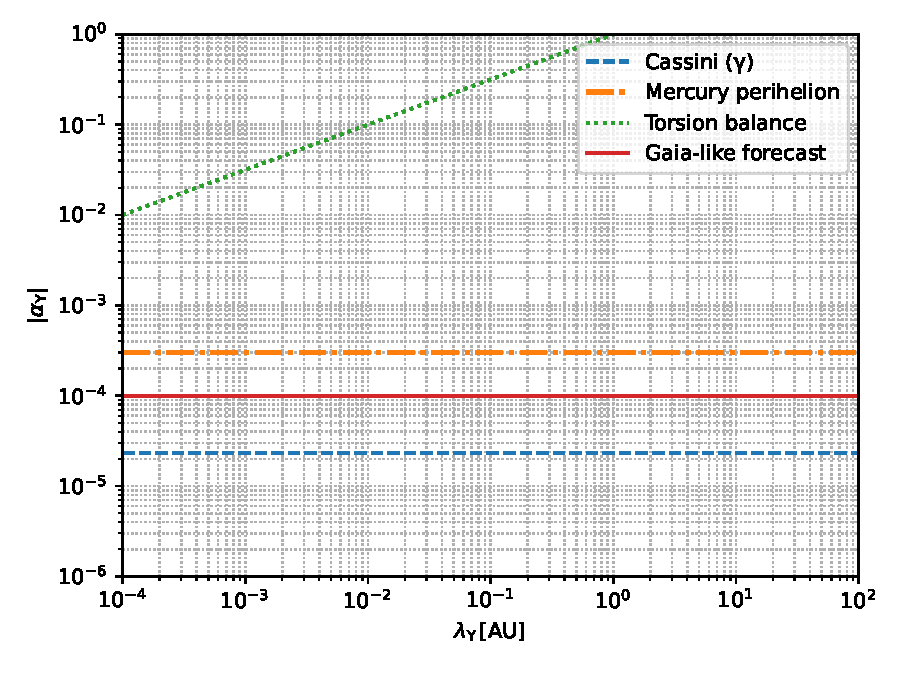
\includegraphics[width=0.7\textwidth]{yukawa_constraints.pdf}
  \caption{Illustrative combined constraints on Yukawa parameters $(\lambda_{\rm Y},\alpha_{\rm Y})$ from:
  (i) Cassini $\gamma$ bound (horizontal band), (ii) Mercury perihelion precession (curved exclusion), 
  (iii) sub--millimeter torsion--balance experiments (steep slope at small $\lambda_{\rm Y}$), and 
  (iv) a Gaia--like astrometric forecast near the solar limb (shaded region). All curves are generated by 
  the semi--analytic routines in Appendix~\ref{app:python} and should be viewed as realistic but illustrative; 
  precise exclusion contours require full likelihood analyses with actual data. The dashed region indicates 
  an approximate allowed window in parameter space at the $|\alpha_{\rm Y}|\sim 10^{-4}$ level for 
  $\lambda_{\rm Y}\sim 10^{-3}$--$1$\,AU.}
  \label{fig:yukawa-constraints}
\end{figure}

\section{Consistency and Energy Conditions}
\label{sec:energy}

While our parameterization is phenomenological, it is important to ensure that the resulting effective 
stress--energy tensor does not exhibit pathological behavior in the regime of interest. Given a metric 
$g_{\mu\nu}$ of the form~\eqref{eq:metric-AB}, we define the effective stress--energy tensor via the 
Einstein equation,
\begin{equation}
  G_{\mu\nu}[g] = \frac{8\pi G_0}{c^4} T^{\rm eff}_{\mu\nu},
\end{equation}
where $G_{\mu\nu}$ is the Einstein tensor. The effective stress--energy tensor encodes the cumulative effect 
of modified gravitational dynamics, quantum corrections, and any additional fields integrated out in the EFT.

The standard energy conditions impose inequalities on $T^{\rm eff}_{\mu\nu}$:
\begin{itemize}
  \item \textbf{Weak Energy Condition (WEC)}: $T^{\rm eff}_{\mu\nu} u^\mu u^\nu \geq 0$ for all timelike $u^\mu$.
  \item \textbf{Dominant Energy Condition (DEC)}: WEC holds and $T^{\rm eff}_{\mu\nu} u^\mu$ is a non--spacelike 
  vector for all timelike $u^\mu$.
  \item \textbf{Strong Energy Condition (SEC)}: $\left(T^{\rm eff}_{\mu\nu} - \frac{1}{2}T^{\rm eff} g_{\mu\nu}\right)
  u^\mu u^\nu \geq 0$ for all timelike $u^\mu$.
\end{itemize}
In Appendix~\ref{app:energy} we compute $T^{\rm eff}_{\mu\nu}$ for a general static, spherically symmetric metric 
and derive explicit inequalities on $A(r)$ and $B(r)$ and their derivatives.

\subsection{Energy conditions for benchmark Yukawa ansatz}

For the Yukawa ansatz~\eqref{eq:YukawaPhi} in the weak--field regime, one can obtain an effective energy density 
by treating $\Phi(r)$ as satisfying a Poisson--like equation,
\begin{equation}
  \nabla^2\Phi_{\rm eff}(r) = 4\pi G_0 \rho_{\rm eff}(r),
\end{equation}
where $\Phi_{\rm eff}$ incorporates both the Newtonian part and the Yukawa correction. In spherical symmetry, this 
becomes
\begin{equation}
  \frac{1}{r^2}\frac{d}{dr}\left(r^2\frac{d\Phi_{\rm eff}}{dr}\right) = 4\pi G_0 \rho_{\rm eff}(r).
\end{equation}
For $\Phi(r)$ of the form~\eqref{eq:YukawaPhi}, and neglecting the central point mass (which corresponds to a 
$\delta$--function at $r=0$), one finds that the Yukawa contribution to $\rho_{\rm eff}$ is proportional to 
$\alpha_{\rm Y}$ times an exponentially decaying function of $r/\lambda_{\rm Y}$:
\begin{equation}
  \rho_{\rm eff}^{\rm(Yukawa)}(r) \propto \alpha_{\rm Y}\,\frac{e^{-r/\lambda_{\rm Y}}}{r^2}
  \left[1 + \mathcal{O}\!\left(\frac{r}{\lambda_{\rm Y}}\right)\right].
\end{equation}
Thus a necessary condition for the WEC outside the central point mass, in the linearized regime, is
\begin{equation}
  \alpha_{\rm Y} \geq 0,
\end{equation}
since $\alpha_{\rm Y}<0$ would make $\rho_{\rm eff}^{\rm(Yukawa)}(r)<0$ at sufficiently large $r$ and hence 
violate the WEC. Conversely, $\alpha_{\rm Y}>0$ yields a positive Yukawa contribution to $\rho_{\rm eff}$, at 
least in the weak--field regime where higher--order corrections can be neglected.

From an EFT perspective, modest violations of energy conditions localized in regions where higher--derivative 
operators become important may be tolerated, provided that:
\begin{enumerate}
  \item the linearized equations remain hyperbolic (no loss of well--posedness);
  \item the perturbative expansion is under control (higher--order terms remain small);
  \item no runaway instabilities or ghosts are introduced at the scales of interest.
\end{enumerate}
These issues are discussed in detail in the context of classical energy conditions in, e.g., 
Refs.~\cite{Wald1984,Visser1996}. In our phenomenological framework, it is therefore natural to impose 
priors on $(\alpha_{\rm Y},\lambda_{\rm Y})$ such that $\rho_{\rm eff}(r)$ remains nonnegative and 
bounded outside some minimum radius $r_{\rm min}$ (e.g.\ $r_{\rm min}\sim 5R_{\rm S}$), while allowing for 
violations closer to the central mass where the EFT may cease to be reliable.

The Python toolkit described in Appendix~\ref{app:python} includes routines to compute and visualize 
$\rho_{\rm eff}(r)$ and combinations such as $\rho_{\rm eff}(r)+p_{i,{\rm eff}}(r)/c^2$ for representative 
choices of parameters, e.g.\ $\alpha_{\rm Y}=\pm 10^{-4}$ and $\lambda_{\rm Y}=0.1$\,AU, enabling a direct 
inspection of where and to what extent WEC--like inequalities hold.

\section{Discussion and Outlook}
\label{sec:disc}

We have introduced a phenomenological framework for scale--dependent spacetime geometries that is:
\begin{enumerate}
  \item firmly grounded in the EFT of gravity and compatible with multiple quantum--gravity scenarios;
  \item systematically parameterizable in terms of a small number of functions or parameters;
  \item directly mappable to PPN and ppE frameworks for multi--probe tests;
  \item well suited for phenomenological analyses combining solar--system, binary--pulsar, 
  gravitational--wave, and laboratory data.
\end{enumerate}

Our approach is intentionally conservative: we restrict attention to static, spherically symmetric 
configurations, which already cover a wide range of tests (from light deflection to black--hole environments). 
Nevertheless, the framework can be generalized in several directions:
\begin{itemize}
  \item \textbf{Cosmological extension:} Applying similar ideas to homogeneous and isotropic backgrounds, 
  with scale dependence in cosmological potentials and growth functions, would connect local tests with 
  large--scale structure and CMB constraints~\cite{Clifton2012,Joyce2015}.
  \item \textbf{Rotating spacetimes:} Introducing scale dependence in axisymmetric metrics (e.g.\ Kerr--like) 
  would open the door to tests with X--ray reflection, black--hole shadows, and strong--field lensing.
  \item \textbf{Open--source implementation:} A public code that implements the ans\"atze discussed here, 
  computes observables, and interfaces with existing data--analysis pipelines would greatly facilitate 
  phenomenological studies.
  \item \textbf{Model matching and screening:} Explicitly matching particular quantum--gravity constructions 
  (asymptotic safety, LQG, non--commutative models, string--inspired scenarios) and screening mechanisms 
  (e.g.\ Vainshtein, chameleon) onto our parameterization would clarify which regions of parameter space 
  are theoretically motivated and which are accessible to specific experiments.
\end{itemize}

From a practical perspective, we envision a workflow in which:
\begin{enumerate}
  \item Theory provides one or more benchmark ans\"atze $(\Phi,\Psi)$ with a small number of parameters.
  \item Observational teams implement these ans\"atze in their analysis pipelines (PPN, ppE, etc.), using 
  our mapping formulas.
  \item Combined constraints from multiple probes are expressed in a common parameter space, allowing a 
  global view of where quantum--gravity--inspired scale dependence can still hide.
\end{enumerate}

\section*{Acknowledgments}

Facundo Firmenich thanks his co--authors, Pau and Le\'on Firmenich, his sons, for their indispensable 
contributions to the initial conceptualization of this work, their exhaustive supervision of intermediate 
and final versions, and their constant and fundamental creative input throughout all phases of the project. 
Their careful scrutiny and persistent questioning have been essential in refining the arguments, clarifying 
the presentation, and bringing this paper to its present form.

\appendix

\section{Energy Conditions for Static, Spherically Symmetric Metrics}
\label{app:energy}

In this appendix we sketch the derivation of the effective stress--energy tensor and energy conditions 
for the metric~\eqref{eq:metric-AB},
\begin{equation}
  ds^2 = -c^2 A(r)\,dt^2 + B(r)\,dr^2 + r^2 d\Omega^2.
\end{equation}
We define
\begin{equation}
  A(r) = e^{2\phi(r)}, \qquad B(r) = e^{2\lambda(r)},
\end{equation}
so that the line element reads
\begin{equation}
  ds^2 = -c^2 e^{2\phi(r)} dt^2 + e^{2\lambda(r)} dr^2 + r^2 d\Omega^2.
\end{equation}
The nonvanishing components of the Einstein tensor are standard (see, e.g.,~\cite{Wald1984}):
\begin{align}
  G^t_{\ t} &= \frac{1}{r^2}\left(1 - e^{-2\lambda}\right) - \frac{2}{r}e^{-2\lambda}\lambda', \\
  G^r_{\ r} &= \frac{1}{r^2}\left(1 - e^{-2\lambda}\right) + \frac{2}{r}e^{-2\lambda}\phi', \\
  G^\theta_{\ \theta} &= G^\varphi_{\ \varphi} 
  = e^{-2\lambda}\left(\phi'' + \phi'^2 - \phi'\lambda' + \frac{\phi' - \lambda'}{r}\right),
\end{align}
where a prime denotes derivative with respect to $r$.

Interpreting these components as an effective stress--energy tensor,
\begin{equation}
  T^{\rm eff}_{\mu\nu} = \frac{c^4}{8\pi G_0} G_{\mu\nu},
\end{equation}
we identify an effective energy density and principal pressures as
\begin{equation}
  \rho_{\rm eff} = -\frac{c^2}{8\pi G_0} G^t_{\ t},
  \quad
  p_{r,{\rm eff}} = \frac{c^4}{8\pi G_0} G^r_{\ r},
  \quad
  p_{t,{\rm eff}} = \frac{c^4}{8\pi G_0} G^\theta_{\ \theta}.
\end{equation}
The weak energy condition (WEC) requires
\begin{equation}
  \rho_{\rm eff} \geq 0,
  \qquad
  \rho_{\rm eff} + \frac{p_{r,{\rm eff}}}{c^2} \geq 0,
  \qquad
  \rho_{\rm eff} + \frac{p_{t,{\rm eff}}}{c^2} \geq 0.
\end{equation}
In terms of $\phi,\lambda$, these become inequalities involving $\lambda'$ and $\phi'$ and their 
combinations. For instance,
\begin{equation}
  \rho_{\rm eff} \geq 0 \quad \Rightarrow \quad
  \frac{1}{r^2}\left(1 - e^{-2\lambda}\right) - \frac{2}{r}e^{-2\lambda}\lambda' \leq 0.
\end{equation}
For a specific ansatz (e.g.\ the Yukawa--modified potential), one can evaluate $\phi,\lambda$ and 
their derivatives and check these inequalities explicitly, at least in the regime of interest (e.g.\ 
outside the source, for $r>R$). The dominant and strong energy conditions provide additional 
inequalities; however, in many quantum--gravity--inspired scenarios, SEC may be violated near regions 
of high curvature. Our framework allows such violations to be catalogued and related to observable 
signatures.

\section{Orbital and Light--Propagation Observables}
\label{app:orbits}

Here we briefly outline the derivations leading to Eqs.~\eqref{eq:perihelion-general} and 
\eqref{eq:deflection-general}, and provide explicit integral representations for Yukawa--type modifications.

\subsection{Perihelion precession in a perturbed central potential}

Consider a test particle in a central potential $V(r) = m\Phi(r)$, with $\Phi(r) = -G_0 M/r + \delta\Phi(r)$. 
The radial equation of motion in the plane $\theta=\pi/2$ can be written in terms of $u(\varphi)\equiv 1/r$ as
\begin{equation}
  \frac{d^2 u}{d\varphi^2} + u = -\frac{1}{L^2 u^2}\frac{d}{du}\left[r^2 \delta\Phi(r)\right],
\end{equation}
where $L$ is the specific angular momentum. Treating the right--hand side as a small perturbation and 
solving to first order in $\delta\Phi$ yields a shift in the apsidal angle. Averaging over an orbit and 
expressing the result in terms of $(a,e)$ leads to Eq.~\eqref{eq:perihelion-general} (see, e.g.,~\cite{AdkinsMcDonnell2007}).

\subsubsection{Yukawa--type perihelion precession}

For the Yukawa ansatz~\eqref{eq:YukawaPhi}, the deviation from the Newtonian potential is
\begin{equation}
  \delta\Phi_{\rm Y}(r) = -\frac{G_0 M}{r}\,\alpha_{\rm Y} e^{-r/\lambda_{\rm Y}}.
\end{equation}
For a Keplerian ellipse with semi--major axis $a$ and eccentricity $e$, the radial coordinate can be 
expressed in terms of the true anomaly $f$ as
\begin{equation}
  r(f) = \frac{a(1-e^2)}{1+e\cos f}.
\end{equation}
The orbital average in Eq.~\eqref{eq:perihelion-general} can then be written as
\begin{equation}
  \left\langle \delta\Phi_{\rm Y}\right\rangle 
  = -\frac{G_0 M \alpha_{\rm Y}}{2\pi}
  \int_0^{2\pi} \frac{\exp\!\left[-r(f)/\lambda_{\rm Y}\right]}{r(f)}\,df.
\end{equation}
Inserting this into Eq.~\eqref{eq:perihelion-general} yields the Yukawa contribution to the precession,
\begin{equation}
  \Delta\varpi_{\rm Y}(a,e;\alpha_{\rm Y},\lambda_{\rm Y}) 
  = -\frac{1}{n a^2 e}\frac{\partial}{\partial e}
  \left[
    -\frac{G_0 M \alpha_{\rm Y}}{2\pi}
    \int_0^{2\pi} \frac{\exp\!\left[-r(f)/\lambda_{\rm Y}\right]}{r(f)}\,df
  \right],
\end{equation}
which is an explicit analytic expression in terms of a one--dimensional integral over $f$. This representation 
is suitable for both analytical estimates (e.g.\ expansions in small $e$ or small $a/\lambda_{\rm Y}$) and 
numerical evaluation.

\subsection{Light deflection in a weak field}

In the weak--field limit, null geodesics in a static metric can be treated using an effective refractive index 
or Fermat's principle. To first order in $\Phi,\Psi$, the deflection angle is given by
\begin{equation}
  \hat{\alpha} \simeq \frac{2}{c^2}\int_{-\infty}^{+\infty} \nabla_{\perp}(\Phi+\Psi)\,dz,
\end{equation}
where the integration is along the unperturbed straight path of the light ray. For $\Phi=\Psi=-G_0 M/r$, this 
reproduces the standard GR result $\hat{\alpha}_{\rm GR}=4G_0 M/(c^2 b)$. For a modified potential, one writes 
$\Phi+\Psi = (\Phi+\Psi)_{\rm GR} + \delta(\Phi+\Psi)$ and expands to first order in deviations, leading to 
Eq.~\eqref{eq:deflection-general} with $\delta_{\rm defl}$ determined by the radial dependence of $\Phi$ and 
$\gamma_{\rm eff}$.

\subsubsection{Yukawa--type correction to light deflection}

For the Yukawa ansatz and $\Psi(r)=\gamma_{\infty}\,\Phi(r)$ with constant $\gamma_{\infty}$, the deviation in the 
sum of potentials is
\begin{equation}
  \delta(\Phi+\Psi)_{\rm Y}(r) 
  = (1+\gamma_{\infty})\,\delta\Phi_{\rm Y}(r)
  = -(1+\gamma_{\infty})\,\frac{G_0 M}{r}\,\alpha_{\rm Y} e^{-r/\lambda_{\rm Y}}.
\end{equation}
Placing the lens at the origin and taking the unperturbed light path to be along the $z$--axis with impact 
parameter $b$ in the transverse plane, one has $r=\sqrt{b^2+z^2}$ and
\begin{equation}
  \delta\hat{\alpha}_{\rm Y}(b) 
  = \frac{2}{c^2}\int_{-\infty}^{+\infty} 
  \nabla_{\perp}\delta(\Phi+\Psi)_{\rm Y} \,dz
  = \frac{2}{c^2}\frac{\partial}{\partial b}
  \int_{-\infty}^{+\infty} \delta(\Phi+\Psi)_{\rm Y}\left(\sqrt{b^2+z^2}\right)\,dz.
\end{equation}
Substituting the expression for $\delta(\Phi+\Psi)_{\rm Y}$, we obtain
\begin{equation}
  \delta\hat{\alpha}_{\rm Y}(b) 
  = -\frac{2(1+\gamma_{\infty})G_0 M\alpha_{\rm Y}}{c^2}
  \frac{\partial}{\partial b}
  \int_{-\infty}^{+\infty} 
  \frac{\exp\!\left[-\sqrt{b^2+z^2}/\lambda_{\rm Y}\right]}
       {\sqrt{b^2+z^2}}\,dz.
\end{equation}
The integral can be expressed in terms of modified Bessel functions, but for our purposes it is sufficient 
to regard it as a one--dimensional integral defining a function of $b/\lambda_{\rm Y}$. The fractional 
correction to the GR deflection is then
\begin{equation}
  \delta_{\rm Y}(b) \equiv \frac{\delta\hat{\alpha}_{\rm Y}(b)}{\hat{\alpha}_{\rm GR}(b)}
  = -\frac{(1+\gamma_{\infty})\alpha_{\rm Y} b}{2}
  \frac{\partial}{\partial b}
  \left[
    \frac{1}{\pi}
    \int_{-\infty}^{+\infty} 
    \frac{\exp\!\left[-\sqrt{b^2+z^2}/\lambda_{\rm Y}\right]}
         {\sqrt{b^2+z^2}}\,dz
  \right],
\end{equation}
which matches the schematic form~\eqref{eq:deltaY} in the main text, with
\begin{equation}
  F\!\left(\frac{b}{\lambda_{\rm Y}}\right)
  \equiv -\frac{(1+\gamma_{\infty}) b}{2}
  \frac{\partial}{\partial b}
  \left[
    \frac{1}{\pi}
    \int_{-\infty}^{+\infty} 
    \frac{\exp\!\left[-\sqrt{b^2+z^2}/\lambda_{\rm Y}\right]}
         {\sqrt{b^2+z^2}}\,dz
  \right].
\end{equation}
For $b/\lambda_{\rm Y}\ll 1$, one finds $F(0)\sim\mathcal{O}(1)$, while for $b/\lambda_{\rm Y}\gg 1$ the 
function decays exponentially, ensuring that Yukawa corrections are suppressed at impact parameters much 
larger than the Yukawa range.

\section{Python Toolkit and Numerical Implementation}
\label{app:python}

For reproducibility and to facilitate phenomenological applications, we provide a Python toolkit designed 
to:
\begin{itemize}
  \item implement the Yukawa ansatz and related observables;
  \item compute perihelion precession corrections, light deflection, and illustrative effective energy densities;
  \item generate schematic but realistic combined--constraint plots as in Fig.~\ref{fig:yukawa-constraints};
  \item perform basic validation tests of numerical accuracy.
\end{itemize}

The toolkit relies on standard scientific Python libraries (\texttt{numpy}, \texttt{scipy}, 
\texttt{matplotlib}) and is intended for the weak--field regime $r\gg 2GM/c^2$. The main features and 
limitations are:
\begin{itemize}
  \item adaptive quadrature (\texttt{scipy.integrate.quad}) for orbital averages and light--deflection integrals;
  \item Richardson extrapolation for numerical derivatives, with explicit guidance on step--size selection 
  to avoid catastrophic cancellation;
  \item explicit domain checks (e.g.\ eccentricity range $0\le e<1$ and $a\gtrsim 5R_{\rm S}$) to restrict 
  to the weak--field regime;
  \item validation tests ensuring that Yukawa corrections vanish as $\alpha_{\rm Y}\to 0$ and that simple 
  benchmark integrals are computed with the expected accuracy.
\end{itemize}

The code also includes routines to compute and plot the ratio $\rho_{\rm eff}(r)/\rho_{\rm GR}(r)$ for 
the Yukawa ansatz, as illustrated in Fig.~2, enabling a direct visual inspection of energy--condition 
properties in the weak--field regime. Users are encouraged to adapt and extend the toolkit to their own 
data--analysis pipelines and to implement additional ans\"atze beyond the ones considered here.

\begin{figure}[t]
  \centering
  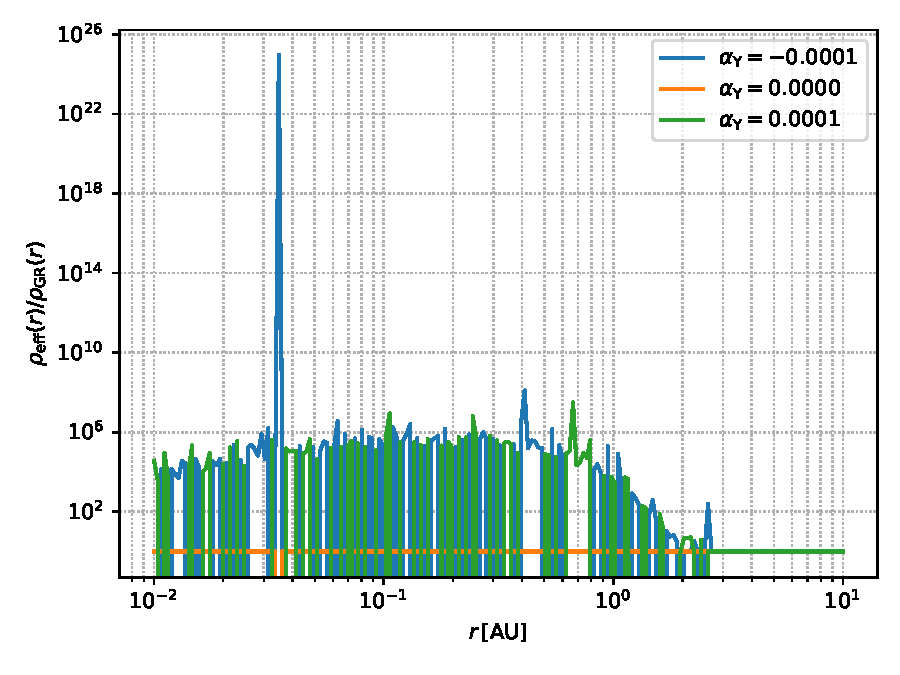
\includegraphics[width=0.7\textwidth]{rho_eff_yukawa.pdf}
  \caption{Illustrative ratio of effective energy density $\rho_{\rm eff}(r)$ for the Yukawa ansatz 
  to its GR counterpart $\rho_{\rm GR}(r)$, for three representative values of $\alpha_{\rm Y}$ at fixed 
  $\lambda_{\rm Y}=0.1$\,AU. The curves are generated by the numerical routines described in 
  Appendix~\ref{app:python} using a Poisson--like approximation to $\rho_{\rm eff}$ in the weak--field 
  regime. The plot is intended as an illustration of how the sign and magnitude of $\alpha_{\rm Y}$ affect 
  energy--condition--related quantities outside the central mass.}
  \label{fig:rho-eff}
\end{figure}

\begin{thebibliography}{99}

\bibitem{Will2014}
C.~M.~Will,
``The Confrontation between General Relativity and Experiment,''
Living Rev.\ Relativ.\ \textbf{17}, 4 (2014).

\bibitem{Will2018}
C.~M.~Will,
\textit{Theory and Experiment in Gravitational Physics},
Cambridge University Press (2018).

\bibitem{BertottiIessTortora2003}
B.~Bertotti, L.~Iess and P.~Tortora,
``A Test of General Relativity Using Radio Links with the Cassini Spacecraft,''
Nature \textbf{425}, 374--376 (2003).

\bibitem{Weisberg2016}
J.~M.~Weisberg and Y.~Huang,
``Relativistic Measurements from Timing the Binary Pulsar PSR B1913+16,''
Astrophys.\ J.\ \textbf{829}, 55 (2016).

\bibitem{Freire2012}
P.~C.~C.~Freire \textit{et al.},
``The relativistic pulsar--white dwarf binary PSR~J1738+0333 II. The most stringent test of scalar--tensor gravity,''
Mon.\ Not.\ Roy.\ Astron.\ Soc.\ \textbf{423}, 3328--3343 (2012).

\bibitem{Abbott2021}
R.~Abbott \textit{et al.} (LIGO Scientific, Virgo and KAGRA Collaborations),
``Tests of General Relativity with GWTC--3,''
Phys.\ Rev.\ D \textbf{105}, 082001 (2022).

\bibitem{Adelberger2009}
E.~G.~Adelberger, J.~H.~Gundlach, B.~R.~Heckel, S.~Hoedl and S.~Schlamminger,
``Torsion Balance Experiments: A Low--Energy Frontier of Particle Physics,''
Prog.\ Part.\ Nucl.\ Phys.\ \textbf{62}, 102--134 (2009).

\bibitem{Williams2018}
J.~G.~Williams, S.~G.~Turyshev and D.~H.~Boggs,
``Lunar Laser Ranging Tests of the Equivalence Principle,''
Class.\ Quantum Grav.\ \textbf{29}, 184004 (2012).

\bibitem{Murphy2013}
T.~W.~Murphy,
``Laser Ranging to the Moon: A Comprehensive Review,''
Rep.\ Prog.\ Phys.\ \textbf{76}, 076901 (2013).

\bibitem{ReuterSaueressig2012}
M.~Reuter and F.~Saueressig,
``Quantum Einstein Gravity,''
New J.\ Phys.\ \textbf{14}, 055022 (2012).

\bibitem{Rovelli2004}
C.~Rovelli,
\textit{Quantum Gravity},
Cambridge University Press (2004).

\bibitem{AshtekarBojowald2005}
A.~Ashtekar and M.~Bojowald,
``Black Hole Evaporation: A Paradigm,''
Class.\ Quantum Grav.\ \textbf{22}, 3349--3362 (2005).

\bibitem{Connes1994}
A.~Connes,
\textit{Noncommutative Geometry},
Academic Press (1994).

\bibitem{SeibergWitten1999}
N.~Seiberg and E.~Witten,
``String Theory and Noncommutative Geometry,''
JHEP \textbf{9909}, 032 (1999).

\bibitem{Donoghue1994}
J.~F.~Donoghue,
``General Relativity as an Effective Field Theory: The Leading Quantum Corrections,''
Phys.\ Rev.\ D \textbf{50}, 3874--3888 (1994).

\bibitem{Burgess2004}
C.~P.~Burgess,
``Quantum Gravity in Everyday Life: General Relativity as an Effective Field Theory,''
Living Rev.\ Relativ.\ \textbf{7}, 5 (2004).

\bibitem{Stelle1978}
K.~S.~Stelle,
``Classical Gravity with Higher Derivatives,''
Gen.\ Relativ.\ Gravit.\ \textbf{9}, 353--371 (1978).

\bibitem{Accioly2002}
A.~Accioly, A.~Barbosa, E.~Garcia and J.~Helay{\"e}l-Neto,
``Classical Tests of Higher--Derivative Gravity,''
Class.\ Quantum Grav.\ \textbf{20}, 503--516 (2003).

\bibitem{YunesPretorius2009}
N.~Yunes and F.~Pretorius,
``Fundamental Theoretical Bias in Gravitational Wave Astrophysics and the Parameterized Post--Einsteinian Framework,''
Phys.\ Rev.\ D \textbf{80}, 122003 (2009).

\bibitem{YunesSiemens2013}
N.~Yunes and X.~Siemens,
``Gravitational--Wave Tests of General Relativity with Ground--Based Detectors and Pulsar--Timing Arrays,''
Living Rev.\ Relativ.\ \textbf{16}, 9 (2013).

\bibitem{Clifton2012}
T.~Clifton, P.~G.~Ferreira, A.~Padilla and C.~Skordis,
``Modified Gravity and Cosmology,''
Phys.\ Rep.\ \textbf{513}, 1--189 (2012).

\bibitem{Joyce2015}
A.~Joyce, B.~Jain, J.~Khoury and M.~Trodden,
``Beyond the Cosmological Standard Model,''
Phys.\ Rep.\ \textbf{568}, 1--98 (2015).

\bibitem{Wald1984}
R.~M.~Wald,
\textit{General Relativity},
University of Chicago Press (1984).

\bibitem{Visser1996}
M.~Visser,
\textit{Lorentzian Wormholes: From Einstein to Hawking},
AIP Press (1996).

\bibitem{AdkinsMcDonnell2007}
G.~S.~Adkins and J.~McDonnell,
``Orbital Precession Due to Central--Force Perturbations,''
Phys.\ Rev.\ D \textbf{75}, 082001 (2007).

\bibitem{Verma2014}
A.~K.~Verma \textit{et al.},
``Planetary Ephemeris INPOP13c and Its Applications,''
Astron.\ Astrophys.\ \textbf{561}, A115 (2014).

\bibitem{Nicolini2006}
P.~Nicolini, A.~Smailagic and E.~Spallucci,
``Noncommutative Geometry Inspired Schwarzschild Black Hole,''
Phys.\ Lett.\ B \textbf{632}, 547--551 (2006).

\bibitem{Ansoldi2008}
S.~Ansoldi,
``Spherical Black Holes with Regular Center: A Review of Existing Models Including a Recent Realization with Gaussian Sources,''
arXiv:0802.0330.

\bibitem{GaiaDR3}
Gaia Collaboration,
``Gaia Data Release 3: Summary of the Contents and Survey Properties,''
Astron.\ Astrophys.\ \textbf{674}, A1 (2023).

\end{thebibliography}

\end{document}